\documentclass[aspectratio=169, 10pt]{beamer}

% ===================== THEME & COLORS =====================
\usetheme{Madrid}
\usecolortheme{default}

\definecolor{minesblue}{RGB}{27,79,114}
\definecolor{minesdark}{RGB}{20,55,80}
\definecolor{mineslight}{RGB}{214,234,248}
\definecolor{accentgreen}{RGB}{39,174,96}
\definecolor{accentorange}{RGB}{243,156,18}
\definecolor{accentred}{RGB}{231,76,60}

\setbeamercolor{palette primary}{bg=minesblue, fg=white}
\setbeamercolor{palette secondary}{bg=minesdark, fg=white}
\setbeamercolor{palette tertiary}{bg=minesdark, fg=white}
\setbeamercolor{structure}{fg=minesblue}
\setbeamercolor{title}{fg=white, bg=minesblue}
\setbeamercolor{frametitle}{fg=white, bg=minesblue}
\setbeamercolor{block title}{bg=minesblue, fg=white}
\setbeamercolor{block body}{bg=mineslight, fg=black}
\setbeamercolor{block title alerted}{bg=accentred, fg=white}
\setbeamercolor{block body alerted}{bg=accentred!10, fg=black}
\setbeamercolor{block title example}{bg=accentgreen, fg=white}
\setbeamercolor{block body example}{bg=accentgreen!10, fg=black}
\setbeamercolor{item}{fg=minesblue}

\setbeamertemplate{navigation symbols}{}
\setbeamertemplate{footline}{
  \leavevmode\hbox{%
    \begin{beamercolorbox}[wd=.33\paperwidth,ht=2.5ex,dp=1ex,center]{palette primary}
      \usebeamerfont{author in head/foot}\insertshortauthor
    \end{beamercolorbox}%
    \begin{beamercolorbox}[wd=.34\paperwidth,ht=2.5ex,dp=1ex,center]{palette secondary}
      \usebeamerfont{title in head/foot}\insertshorttitle
    \end{beamercolorbox}%
    \begin{beamercolorbox}[wd=.33\paperwidth,ht=2.5ex,dp=1ex,right]{palette tertiary}
      \usebeamerfont{date in head/foot}\insertframenumber{} / \inserttotalframenumber\hspace*{2em}
    \end{beamercolorbox}}
}

% ===================== PACKAGES =====================
\usepackage[utf8]{inputenc}
\usepackage[T1]{fontenc}
% babel removed - content in French, no hyphenation needed
\usepackage{amsmath,amssymb}
\usepackage{booktabs}
\usepackage{graphicx}
\usepackage{tikz}
\usetikzlibrary{arrows.meta, positioning, shapes.geometric, calc, decorations.pathreplacing}
\usepackage{multicol}
\usepackage{hyperref}

% ===================== TITLE =====================
\title[WAPP DAM --- Revue \& Modélisation]{Développement - outil de simulation - Marché day-ahead du WAPP}
\subtitle{Revue de littérature \& Début de modélisation}
\author[Équipe OSE]{K. Plakoo \quad E. Patanè \quad L. Kouakou \quad M. Sow \quad M.W. Hmila}
\institute[MINES Paris]{Mastère OSE --- MINES Paris-PSL}
\date{13 février 2026}

\begin{document}

% ===================== TITLE PAGE =====================
{
\setbeamertemplate{footline}{}
\begin{frame}[plain]
\vspace{1.2cm}

% === ESPACE POUR LES LOGOS ===
\begin{columns}[c]
  \column{0.5\textwidth}\centering
    \includegraphics[height=1.6cm]{assets/mines_logo.png}
  \column{0.1\textwidth}\centering
  \column{0.5\textwidth}\centering
    \includegraphics[height=1.6cm]{assets/wapp_logo.png}
\end{columns}

\vspace{0.2cm}
\titlepage

\vspace{-0.5cm}
\centering
{\small\color{gray} Supervisé par \textbf{El Hadji Tamsir Diop} (SENELEC)}
\end{frame}
}

% ===================== PLAN =====================
\begin{frame}{Plan}
\tableofcontents
\end{frame}

% ============================================================
\section{Revue de littérature}
% ============================================================

% --- Slide: Contexte WAPP ---
\begin{frame}{Le WAPP --- Contexte}
\begin{columns}[T]
\column{0.55\textwidth}
\begin{itemize}
  \item \textbf{14 pays} de la CEDEAO, \textbf{35+ utilities}
  \item 13/14 réseaux interconnectés (depuis juillet 2023)
  \item ICC inauguré en novembre 2023
  \item Marché day-ahead en cours d'opérationnalisation
  \item Taux d'accès à l'électricité $\sim$52\% (2020)
\end{itemize}

\vspace{0.3cm}
\begin{block}{Objectif du marché}
Permettre des échanges compétitifs J-1 entre zones pour \textbf{réduire les coûts} et \textbf{optimiser les ressources} régionales.
\end{block}

\column{0.42\textwidth}
\centering
% Schéma simplifié du réseau
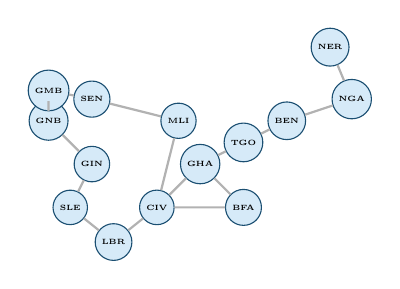
\begin{tikzpicture}[
  scale=0.55, transform shape,
  zone/.style={circle, draw=minesblue, fill=mineslight, minimum size=0.7cm, font=\tiny\bfseries},
  link/.style={draw=gray!60, thick}
]
  \node[zone] (NGA) at (4,3) {NGA};
  \node[zone] (BEN) at (2.5,2.5) {BEN};
  \node[zone] (TGO) at (1.5,2) {TGO};
  \node[zone] (GHA) at (0.5,1.5) {GHA};
  \node[zone] (CIV) at (-0.5,0.5) {CIV};
  \node[zone] (BFA) at (1.5,0.5) {BFA};
  \node[zone] (MLI) at (0,2.5) {MLI};
  \node[zone] (SEN) at (-2,3) {SEN};
  \node[zone] (GIN) at (-2,1.5) {GIN};
  \node[zone] (SLE) at (-2.5,0.5) {SLE};
  \node[zone] (LBR) at (-1.5,-0.3) {LBR};
  \node[zone] (GNB) at (-3,2.5) {GNB};
  \node[zone] (GMB) at (-3,3.2) {GMB};
  \node[zone] (NER) at (3.5,4.2) {NER};

  \foreach \a/\b in {NGA/BEN, NGA/NER, BEN/TGO, TGO/GHA, GHA/CIV, GHA/BFA, CIV/BFA, CIV/MLI, CIV/LBR, LBR/SLE, SLE/GIN, GIN/GNB, GNB/GMB, GMB/SEN, SEN/MLI}
    \draw[link] (\a) -- (\b);
\end{tikzpicture}

\vspace{0.2cm}
{\scriptsize 14 zones $\times$ 15 interconnexions}
\end{columns}
\end{frame}

% --- Slide: Structure du rapport ---
\begin{frame}{Structure de la revue de littérature}
\begin{columns}[T]
\column{0.48\textwidth}
\begin{block}{1. Cadre institutionnel du WAPP}
\begin{itemize}\small
  \item Gouvernance : CEDEAO $\to$ WAPP $\to$ ICC
  \item Régulation : ERERA (pouvoirs contraignants)
  \item Phases de déploiement du marché
  \item Comparaison : SAPP, EAPP, CAPP
\end{itemize}
\end{block}

\begin{block}{2. Design de marché}
\begin{itemize}\small
  \item Approche zonale (NTC) vs nodale (LMP)
  \item Couplage flow-based vs ATC
  \item Expérience européenne (SDAC/EUPHEMIA)
  \item Choix retenu : \textbf{zonal NTC}
\end{itemize}
\end{block}

\column{0.48\textwidth}
\begin{block}{3. Algorithmes de clearing}
\begin{itemize}\small
  \item Maximisation du welfare social
  \item EUPHEMIA : structure et fonctionnement
  \item Non-convexité et ordres paradoxaux
  \item Méthodes de résolution (MILP)
\end{itemize}
\end{block}

\begin{block}{4. Offres complexes}
\begin{itemize}\small
  \item Block orders (fill-or-kill)
  \item Linked orders (parent-enfant)
  \item Groupes exclusifs
  \item Minimum Income Condition (MIC)
\end{itemize}
\end{block}
\end{columns}

\vspace{0.2cm}
\centering {\small\color{gray} $>$75 références $\cdot$ 45 pages $\cdot$ Soumis le 8 février 2026}
\end{frame}

% --- Slide: Design de marché ---
\begin{frame}{Choix de design : approche zonale avec NTC}

\begin{columns}[T]
\column{0.48\textwidth}

\textbf{Pourquoi l'approche zonale ?}
\begin{itemize}\small
  \item Adoptée par le WAPP (inspiré du modèle européen)
  \item 1 zone = 1 pays $\Rightarrow$ 14 zones de prix
  \item Échanges limités par les \textbf{NTC} entre zones
  \item Plus simple que le nodal : pas besoin du modèle réseau complet
\end{itemize}

\vspace{0.3cm}
\textbf{Market splitting}
\begin{itemize}\small
  \item Si NTC non saturé $\Rightarrow$ prix convergent
  \item Si NTC saturé $\Rightarrow$ \textcolor{accentred}{séparation des prix}
  \item Rente de congestion $= (\lambda_v - \lambda_u) \times f_{uv}$
\end{itemize}

\column{0.5\textwidth}
\centering
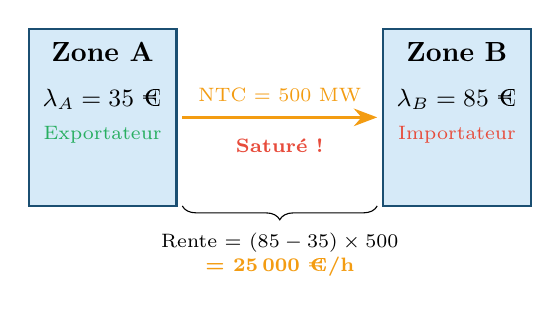
\begin{tikzpicture}[scale=0.75]
  % Zone A
  \draw[thick, minesblue, fill=mineslight] (0,0) rectangle (2.5,3);
  \node[font=\bfseries] at (1.25,2.6) {Zone A};
  \node[font=\small] at (1.25,1.8) {$\lambda_A = 35$ €};
  \node[font=\scriptsize, accentgreen] at (1.25,1.2) {Exportateur};
  
  % Zone B
  \draw[thick, minesblue, fill=mineslight] (6,0) rectangle (8.5,3);
  \node[font=\bfseries] at (7.25,2.6) {Zone B};
  \node[font=\small] at (7.25,1.8) {$\lambda_B = 85$ €};
  \node[font=\scriptsize, accentred] at (7.25,1.2) {Importateur};

  % NTC link
  \draw[-{Stealth}, very thick, accentorange] (2.6,1.5) -- (5.9,1.5);
  \node[above, font=\scriptsize, accentorange] at (4.25,1.6) {NTC = 500 MW};
  \node[below, font=\scriptsize, accentred] at (4.25,1.3) {\textbf{Saturé !}};

  % Congestion rent
  \draw[decorate, decoration={brace, amplitude=5pt, mirror}] (2.6,0) -- (5.9,0);
  \node[below, font=\scriptsize] at (4.25,-0.3) {Rente = $(85-35) \times 500$};
  \node[below, font=\scriptsize\bfseries, accentorange] at (4.25,-0.7) {= 25\,000 €/h};
\end{tikzpicture}
\end{columns}
\end{frame}

% --- Slide: EUPHEMIA ---
\begin{frame}{L'algorithme EUPHEMIA}
\begin{columns}[T]
\column{0.55\textwidth}

\textbf{Algorithme de référence} pour le couplage day-ahead européen (SDAC) :
\begin{enumerate}\small
  \item Collecte des offres de toutes les zones
  \item \textbf{Maximisation du welfare social} (MILP)
  \item Détermination des prix zonaux (variables duales)
  \item Vérification des ordres paradoxaux (PRB/PAB)
  \item Boucle itérative si PAB détectés
\end{enumerate}

\vspace{0.3cm}
\textbf{Défis de la non-convexité} :
\begin{itemize}\small
  \item Les block orders (binaires) rendent le problème non-convexe
  \item Pas de prix d'équilibre « parfait » garanti
  \item Compromis welfare vs nombre de PAB/PRB
\end{itemize}

\column{0.4\textwidth}
\centering
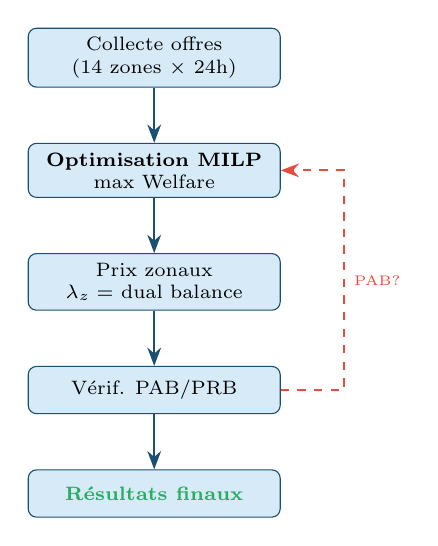
\begin{tikzpicture}[
  node distance=0.7cm,
  box/.style={rectangle, draw=minesblue, fill=mineslight, rounded corners=3pt, minimum width=3.2cm, minimum height=0.6cm, font=\scriptsize, align=center},
  arr/.style={-{Stealth}, thick, minesblue}
]
  \node[box] (col) {Collecte offres\\(14 zones $\times$ 24h)};
  \node[box, below=of col] (opt) {\textbf{Optimisation MILP}\\$\max$ Welfare};
  \node[box, below=of opt] (prix) {Prix zonaux\\$\lambda_z =$ dual balance};
  \node[box, below=of prix] (pao) {Vérif. PAB/PRB};
  \node[box, below=of pao] (res) {\textcolor{accentgreen}{\textbf{Résultats finaux}}};

  \draw[arr] (col) -- (opt);
  \draw[arr] (opt) -- (prix);
  \draw[arr] (prix) -- (pao);
  \draw[arr] (pao) -- (res);
  \draw[arr, accentred, dashed] (pao.east) -- ++(0.8,0) |- node[right, font=\tiny, pos=0.25] {PAB?} (opt.east);
\end{tikzpicture}
\end{columns}
\end{frame}

% --- Slide: Offres complexes ---
\begin{frame}{Typologies d'offres}
\begin{columns}[T]
\column{0.32\textwidth}
\begin{block}{Offres horaires}
\begin{itemize}\scriptsize
  \item 1 prix + 1 quantité par heure
  \item Acceptation partielle possible
  \item $x_i \in [0,1]$
\end{itemize}
\end{block}

\column{0.32\textwidth}
\begin{block}{Block orders}
\begin{itemize}\scriptsize
  \item Multi-heures, prix unique
  \item \textbf{Fill-or-kill} : $y_b \in \{0,1\}$
  \item Profils variables possibles
  \item $\Rightarrow$ non-convexité
\end{itemize}
\end{block}

\column{0.32\textwidth}
\begin{block}{Ordres complexes}
\begin{itemize}\scriptsize
  \item \textbf{Liés} : $y_{child} \leq y_{parent}$
  \item \textbf{Exclusifs} : $\sum y_g \leq 1$
  \item \textbf{MIC} : revenu $\geq$ coût fixe
  \item $\Rightarrow$ boucle itérative
\end{itemize}
\end{block}
\end{columns}

\vspace{0.4cm}
\centering

\begin{tikzpicture}[
  scale=0.9,
  phase/.style={rectangle, rounded corners=5pt, minimum width=3.8cm, minimum height=0.9cm, font=\small, align=center, text=white},
  arr/.style={-{Stealth}, thick, gray}
]
  \node[phase, fill=accentgreen] (p1) at (0,0) {Phase 1\\Offres horaires};
  \node[phase, fill=accentorange] (p2) at (5,0) {Phase 2\\+ Block orders};
  \node[phase, fill=accentred] (p3) at (10,0) {Phase 3\\+ Ordres complexes};
  \draw[arr] (p1) -- (p2);
  \draw[arr] (p2) -- (p3);
\end{tikzpicture}
\end{frame}

% ============================================================
\section{Formulation mathématique}
% ============================================================

% --- Slide: Formulation de base ---
\begin{frame}{Formulation --- Offres horaires multi-zones}

\begin{block}{Ensembles}
\vspace{-0.3cm}
\begin{align*}
\mathcal{Z} &= \{1, \ldots, 14\} \text{ (zones/pays)} &
\mathcal{H} &= \{1, \ldots, 24\} \text{ (heures)} \\
\mathcal{S}_z &: \text{offres de vente dans la zone } z &
\mathcal{D}_z &: \text{demandes d'achat dans la zone } z
\end{align*}
\end{block}

\vspace{-0.2cm}

\begin{block}{Objectif --- Maximisation du welfare social}
\vspace{-0.2cm}
$$\max_{x^s, x^d} \quad \sum_{h \in \mathcal{H}} \left[ \sum_{d \in \mathcal{D}} p_d \, q_{d,h} \, x^d_{d,h} \;-\; \sum_{s \in \mathcal{S}} p_s \, q_{s,h} \, x^s_{s,h} \right]$$
\end{block}

\vspace{-0.2cm}

\small
\textbf{Variables} : $x^s_{s,h} \in [0,1]$ (ratio d'acceptation vente), $x^d_{d,h} \in [0,1]$ (ratio d'acceptation demande), $f_{uv,h} \geq 0$ (flux), $b_{uv,h} \in \{0,1\}$ (direction)

\vspace{0.2cm}
Le \textbf{prix zonal} $\lambda_{z,h}$ émerge comme variable duale de la contrainte d'équilibre $\Rightarrow$ \textit{pas une variable de décision}.
\end{frame}

% --- Slide: Contraintes ---
\begin{frame}{Contraintes}

\begin{block}{Équilibre nodal (par zone et par heure)}
\vspace{-0.2cm}
$$\forall z \in \mathcal{Z},\; \forall h \in \mathcal{H}: \quad \sum_{s \in \mathcal{S}_z} q_{s,h} \, x^s_{s,h} + \underbrace{\sum_{(u,z)} f_{u,z,h} + \sum_{(z,v)} f^r_{z,v,h}}_{\text{imports}} - \underbrace{\sum_{(z,v)} f_{z,v,h} + \sum_{(u,z)} f^r_{u,z,h}}_{\text{exports}} = \sum_{d \in \mathcal{D}_z} q_{d,h} \, x^d_{d,h}$$
\end{block}

\begin{block}{Capacités de transfert (NTC)}
\vspace{-0.2cm}
$$f_{uv,h} \leq \text{NTC}_{uv} \cdot b_{uv,h} \qquad\qquad f^r_{uv,h} \leq \text{NTC}_{uv} \cdot (1 - b_{uv,h})$$
\end{block}

\begin{block}{Bornes}
\vspace{-0.2cm}
$$0 \leq x^s_{s,h} \leq 1 \qquad 0 \leq x^d_{d,h} \leq 1 \qquad b_{uv,h} \in \{0,1\}$$
\end{block}

\vspace{0.2cm}
$\Rightarrow$ Problème \textbf{MILP} (Mixed-Integer Linear Program) : binaires uniquement pour la direction des flux.
\end{frame}

% --- Slide: Extension Block Orders ---
\begin{frame}{Extension --- Block orders}

Un block order $b$ s'étend sur les heures $\mathcal{T}_b = [h_1, h_2]$ avec puissance $q_b$ et prix $p_b$.

\vspace{0.2cm}
\textbf{Variable} : $y_b \in \{0,1\}$ (fill-or-kill)

\begin{block}{Contribution au welfare}
\vspace{-0.3cm}
$$W_{\text{blocks}} = \sum_{b \in \mathcal{B}^D} p_b \, q_b \, |\mathcal{T}_b| \, y_b \;-\; \sum_{b \in \mathcal{B}^S} p_b \, q_b \, |\mathcal{T}_b| \, y_b$$
\end{block}

\begin{block}{Injection dans l'équilibre nodal}
\vspace{-0.3cm}
$$\forall z, h: \quad \text{production}_z(h) \mathrel{+}= \sum_{\substack{b \in \mathcal{B}^S_z \\ h \in \mathcal{T}_b}} q_b \, y_b \qquad \text{consommation}_z(h) \mathrel{+}= \sum_{\substack{b \in \mathcal{B}^D_z \\ h \in \mathcal{T}_b}} q_b \, y_b$$
\end{block}

\begin{block}{Condition d'acceptation (vérification ex post)}
\vspace{-0.3cm}
$$\text{Supply block ``in-the-money''} \iff \frac{1}{|\mathcal{T}_b|}\sum_{h \in \mathcal{T}_b} \lambda_{z,h} \geq p_b$$
\end{block}
\end{frame}

% ============================================================
\section{Implémentation Python}
% ============================================================

% --- Slide: Stack technique ---
\begin{frame}{Stack technique}

\begin{columns}[T]
\column{0.48\textwidth}

\begin{block}{Modélisation}
\begin{description}\small
  \item[Pyomo] Framework d'optimisation algébrique
  \item[GLPK/HiGHS] Solveurs open-source (MILP)
  \item[Gurobi] Solveur académique (performances)
\end{description}
\end{block}

\begin{block}{Données \& Visualisation}
\begin{description}\small
  \item[Pandas] Manipulation des données
  \item[Plotly] Graphiques interactifs
  \item[NumPy] Calcul matriciel
\end{description}
\end{block}

\column{0.48\textwidth}

\begin{block}{Approche progressive}
\centering
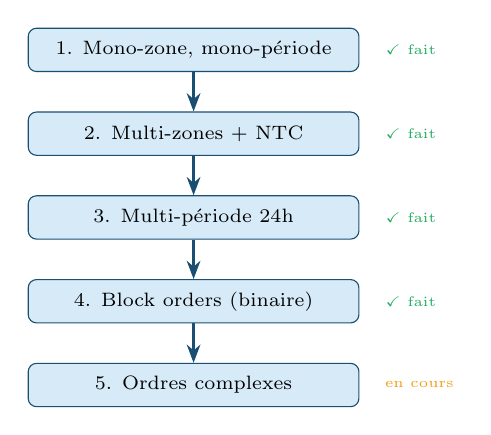
\begin{tikzpicture}[
  node distance=0.5cm,
  stp/.style={rectangle, rounded corners=3pt, draw=minesblue, fill=mineslight, minimum width=4.2cm, minimum height=0.55cm, font=\scriptsize, align=center},
  arr/.style={-{Stealth}, thick, minesblue}
]
  \node[stp] (s1) {1. Mono-zone, mono-période};
  \node[stp, below=of s1] (s2) {2. Multi-zones + NTC};
  \node[stp, below=of s2] (s3) {3. Multi-période 24h};
  \node[stp, below=of s3] (s4) {4. Block orders (binaire)};
  \node[stp, below=of s4] (s5) {5. Ordres complexes};

  \draw[arr] (s1) -- (s2);
  \draw[arr] (s2) -- (s3);
  \draw[arr] (s3) -- (s4);
  \draw[arr] (s4) -- (s5);

  \node[right=0.2cm of s1, font=\tiny, accentgreen] {\checkmark~fait};
  \node[right=0.2cm of s2, font=\tiny, accentgreen] {\checkmark~fait};
  \node[right=0.2cm of s3, font=\tiny, accentgreen] {\checkmark~fait};
  \node[right=0.2cm of s4, font=\tiny, accentgreen] {\checkmark~fait};
  \node[right=0.2cm of s5, font=\tiny, accentorange] {en cours};
\end{tikzpicture}
\end{block}
\end{columns}
\end{frame}

% --- Slide: Résultats préliminaires ---
\begin{frame}{Premiers résultats --- Clearing 24h}

\begin{columns}[T]
\column{0.48\textwidth}

\begin{exampleblock}{Données de test}
\begin{itemize}\small
  \item 28 centrales (solaire, hydro, gaz, peaker)
  \item 15 distributeurs dans les 14 zones
  \item 15 interconnexions avec NTC réalistes
  \item Profils horaires par technologie
\end{itemize}
\end{exampleblock}

\vspace{0.2cm}
\begin{alertblock}{Performances}
\centering
\begin{tabular}{ll}
  Welfare 24h & \textbf{17 980 k€} \\
  Temps résolution & \textbf{$\sim$1 seconde} \\
  Variables & $\sim$2\,400 \\
  Contraintes & $\sim$1\,100 \\
\end{tabular}
\end{alertblock}

\column{0.48\textwidth}

\begin{block}{Observations clés}
\begin{itemize}\small
  \item \textbf{Prix dynamiques} : 35 €/MWh (H04, baseload gaz) $\to$ 130 €/MWh (H18, pointe soir)
  \item \textbf{Solaire} dispatché à 100\% (merit order favorable), production nulle H00-H05
  \item \textbf{Congestions récurrentes} sur NGA$\to$BEN et TGO$\to$GHA
  \item \textbf{Nigeria} : exportateur structurel grâce au gaz bon marché
  \item \textbf{Niger, Burkina} : prix élevés, importateurs nets
\end{itemize}
\end{block}
\end{columns}
\end{frame}

% --- Slide: Profils et dispatch ---
\begin{frame}{Profils de production et dispatch}

\begin{columns}[T]
\column{0.48\textwidth}

\textbf{Profils de disponibilité (normalisés)} :

\vspace{0.2cm}
\centering
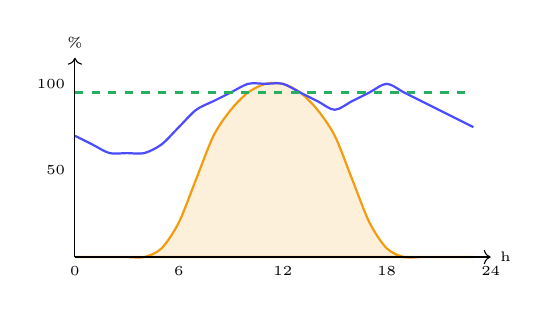
\begin{tikzpicture}[xscale=0.22, yscale=2.2]
  % Solar
  \draw[thick, accentorange, fill=accentorange!15] 
    plot[smooth] coordinates {
      (0,0)(1,0)(2,0)(3,0)(4,0)(5,0.05)(6,0.2)(7,0.45)(8,0.7)(9,0.85)(10,0.95)(11,1)
      (12,1)(13,0.95)(14,0.85)(15,0.7)(16,0.45)(17,0.2)(18,0.05)(19,0)(20,0)(21,0)(22,0)(23,0)
    } -- (23,0) -- (0,0) -- cycle;
  
  % Hydro
  \draw[thick, blue!70] 
    plot[smooth] coordinates {
      (0,0.7)(1,0.65)(2,0.6)(3,0.6)(4,0.6)(5,0.65)(6,0.75)(7,0.85)(8,0.9)(9,0.95)(10,1)(11,1)
      (12,1)(13,0.95)(14,0.9)(15,0.85)(16,0.9)(17,0.95)(18,1)(19,0.95)(20,0.9)(21,0.85)(22,0.8)(23,0.75)
    };
  
  % Baseload
  \draw[thick, accentgreen, dashed] (0,0.95) -- (23,0.95);

  % Axes
  \draw[->] (0,0) -- (24,0) node[right, font=\tiny] {h};
  \draw[->] (0,0) -- (0,1.15) node[above, font=\tiny] {\%};
  \foreach \x in {0,6,12,18,24} \node[below, font=\tiny] at (\x,0) {\x};
  \foreach \y/\l in {0.5/50, 1.0/100} \node[left, font=\tiny] at (0,\y) {\l};
\end{tikzpicture}

\vspace{0.1cm}
{\scriptsize \textcolor{accentorange}{$\blacksquare$ Solaire} \quad \textcolor{blue!70}{--- Hydro} \quad \textcolor{accentgreen}{-- Baseload}}

\column{0.48\textwidth}

\textbf{Courbe de charge Afrique de l'Ouest} :

\vspace{0.2cm}
\centering
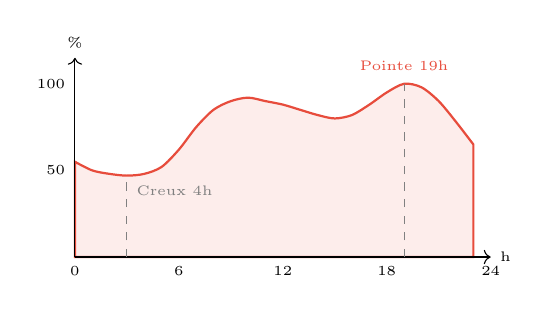
\begin{tikzpicture}[xscale=0.22, yscale=2.2]
  \draw[thick, accentred, fill=accentred!10] 
    plot[smooth] coordinates {
      (0,0.55)(1,0.50)(2,0.48)(3,0.47)(4,0.48)(5,0.52)(6,0.62)(7,0.75)(8,0.85)(9,0.90)
      (10,0.92)(11,0.90)(12,0.88)(13,0.85)(14,0.82)(15,0.80)(16,0.82)(17,0.88)(18,0.95)
      (19,1.0)(20,0.98)(21,0.90)(22,0.78)(23,0.65)
    } -- (23,0) -- (0,0) -- cycle;

  \draw[->] (0,0) -- (24,0) node[right, font=\tiny] {h};
  \draw[->] (0,0) -- (0,1.15) node[above, font=\tiny] {\%};
  \foreach \x in {0,6,12,18,24} \node[below, font=\tiny] at (\x,0) {\x};
  \foreach \y/\l in {0.5/50, 1.0/100} \node[left, font=\tiny] at (0,\y) {\l};
  
  \draw[dashed, gray] (19,0) -- (19,1.0);
  \node[above, font=\tiny, accentred] at (19,1.02) {Pointe 19h};
  
  \draw[dashed, gray] (3,0) -- (3,0.47);
  \node[below right, font=\tiny, gray] at (3,0.47) {Creux 4h};
\end{tikzpicture}

\vspace{0.1cm}
{\scriptsize Creux nocturne ($\sim$47\%) $\to$ pointe soir (100\%)}
\end{columns}

\end{frame}

% --- Slide: Prix zonaux résultats ---
\begin{frame}{Prix zonaux --- Dynamique 24h}
\centering

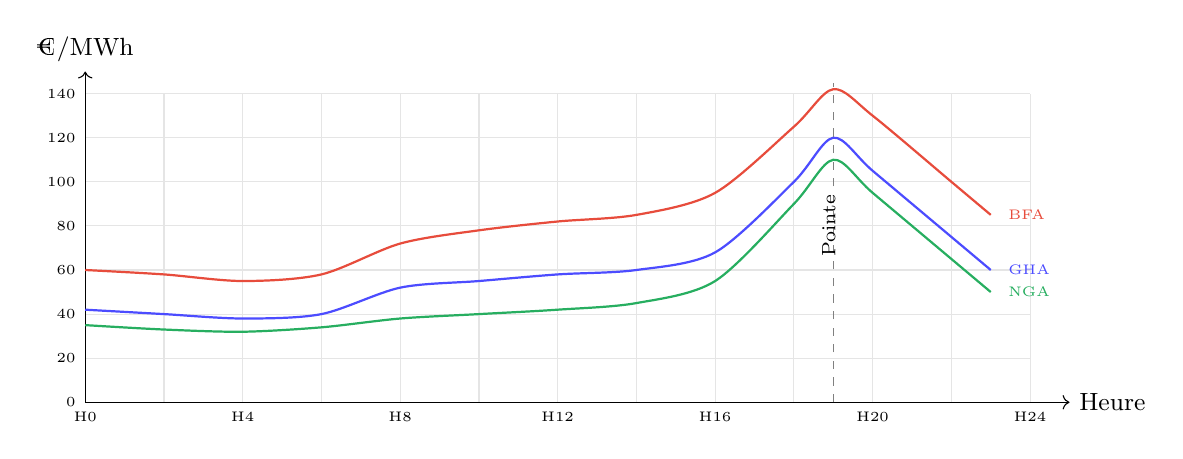
\begin{tikzpicture}[xscale=0.5, yscale=0.028]
  % Grid
  \draw[gray!20] (0,0) grid[xstep=2, ystep=20] (24,140);
  \draw[->] (0,0) -- (25,0) node[right, font=\small] {Heure};
  \draw[->] (0,0) -- (0,150) node[above, font=\small] {€/MWh};
  \foreach \x in {0,4,8,12,16,20,24} \node[below, font=\tiny] at (\x,0) {H\x};
  \foreach \y in {0,20,40,60,80,100,120,140} \node[left, font=\tiny] at (0,\y) {\y};

  % NGA (cheap)
  \draw[thick, accentgreen] plot[smooth] coordinates {
    (0,35)(2,33)(4,32)(6,34)(8,38)(10,40)(12,42)(14,45)(16,55)(18,90)(19,110)(20,95)(22,65)(23,50)};
  \node[right, font=\tiny, accentgreen] at (23.2,50) {NGA};

  % GHA
  \draw[thick, blue!70] plot[smooth] coordinates {
    (0,42)(2,40)(4,38)(6,40)(8,52)(10,55)(12,58)(14,60)(16,68)(18,100)(19,120)(20,105)(22,75)(23,60)};
  \node[right, font=\tiny, blue!70] at (23.2,60) {GHA};

  % BFA (expensive)
  \draw[thick, accentred] plot[smooth] coordinates {
    (0,60)(2,58)(4,55)(6,58)(8,72)(10,78)(12,82)(14,85)(16,95)(18,125)(19,142)(20,130)(22,100)(23,85)};
  \node[right, font=\tiny, accentred] at (23.2,85) {BFA};

  % Annotations
  \draw[dashed, gray] (19,0) -- (19,145);
  \node[above, font=\scriptsize, rotate=90] at (19.3,80) {Pointe};
\end{tikzpicture}

\vspace{0.2cm}
{\small Les prix reflètent le merit order local + les contraintes NTC. Écart NGA--BFA $\sim$50 €/MWh aux heures de pointe $\Rightarrow$ congestion structurelle.}
\end{frame}

% ============================================================
\section{Prochaines étapes}
% ============================================================

\begin{frame}{Planning et prochaines étapes}

\begin{columns}[T]
\column{0.55\textwidth}

\begin{block}{Livrable 2 --- fin février 2026}
\begin{itemize}\small
  \item Formulation mathématique détaillée
  \item Code Python complet avec documentation
  \item Résultats de simulation : 14 zones $\times$ 24h
  \item Intégration block orders validée
  \item Analyse de sensibilité (NTC, mix énergétique)
\end{itemize}
\end{block}

\begin{block}{Livrable 3 --- fin mars 2026}
\begin{itemize}\small
  \item Ordres complexes (linked, exclusive, MIC)
  \item Interface utilisateur interactive (Streamlit)
  \item Scénarios : import/export CSV, paramétrage
  \item Étude de cas complète sur le réseau WAPP
  \item Rapport final et soutenance
\end{itemize}
\end{block}

\column{0.4\textwidth}

\begin{block}{Points de discussion}
\begin{enumerate}\small
  \item Données NTC réelles à intégrer ?
  \item Niveau de détail des offres complexes pour le livrable final ?
  \item Scénarios prioritaires à simuler ?
  \item Quid des données de capacité installée par zone ?
\end{enumerate}
\end{block}

\vspace{0.3cm}
\centering

\begin{tikzpicture}
\node[rectangle, rounded corners=8pt, draw=accentgreen, fill=accentgreen!10, 
  minimum width=4cm, minimum height=1.2cm, align=center, font=\small] {
  \textbf{Code disponible}\\
  Notebook Jupyter\\
  exécutable
};
\end{tikzpicture}

\end{columns}
\end{frame}

% ===================== MERCI =====================
{
\setbeamertemplate{footline}{}
\begin{frame}[plain]
\vfill
\centering

{\Huge\color{minesblue}\textbf{Merci !}}

\vspace{1cm}
{\large Questions \& Discussion}

\vspace{1cm}
{\small\color{gray}
K. Plakoo $\cdot$ E. Patanè $\cdot$ L. Kouakou $\cdot$ M. Sow $\cdot$ M.W. Hmila\\[0.3cm]
Mastère OSE --- MINES Paris-PSL\\[0.2cm]
Superviseur : El Hadji Tamsir Diop (SENELEC)
}

\vfill
\end{frame}
}

\end{document}